\documentclass[a4paper, 12pt]{article}

\usepackage[T1]{fontenc}
\usepackage[polish]{babel} 
\usepackage[utf8]{inputenc} 
\usepackage{indentfirst}
\let\lll\undefined
\usepackage{amssymb}
\usepackage{setspace}
\usepackage{fancyhdr}
\usepackage{graphicx} 

\pagestyle{fancy} 
\newcommand{\mainmatter}{\clearpage \cfoot{\thepage\ of \pageref{LastPage}}
\pagenumbering{arabic}}




\begin{document}
	\begin{titlepage}
		
		\begin{center}
    	\vspace{5cm}
    		\Large\textit{\textbf{SPECYFIKACJA IMPLEMENTACYJNA 
    		\\''Gra w życie'' DLA JĘZYKA PROGROMOWANIA C}}\\ 
		\vspace{15cm}
		\end{center} 

		\hfill\begin{minipage}{0.5\textwidth}
			\Large Wykonali:\newline
				1. Ivan Prakapets \newline
		\vspace{\baselineskip}
		\end{minipage}
		

	\end{titlepage}
\newpage
\mainmatter
\setlength{\headheight}{15pt}
\doublespacing
\tableofcontents
\newpage

	\section{Diagram modułów}
		\begin{figure}[h]
			\center{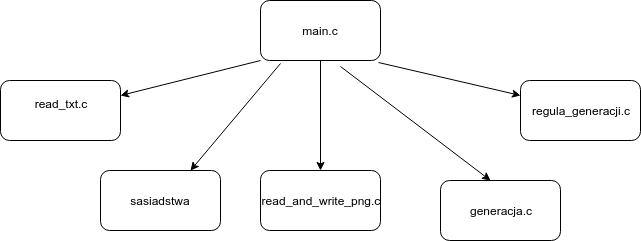
\includegraphics[width=1\linewidth]{diagram}}	
			\caption{Diagram modułów}
		\end{figure}		
			\hspace*{1cm} \newline
			\subsection{Opis diagrama} 
			\hspace*{1cm} Poniżej jest przedstawiony opis diagrama:\newline
			\texttt{main} jest głównym plikiem z rozszerzeniem \texttt{.c}. Plik \texttt{main.c} wiąże między sobą wszystkie poszeczególne moduły w programie ''Gram w życie''. 
\newpage
	\section{Opis i spis funkcji}
		\subsection{Moduł read$\_$and$\_$write$\_$png} 
			\hspace*{1cm} Moduł \texttt{read$\_$and$\_$write$\_$png} składa się z trzech funkcji:
			\renewcommand{\labelitemi}{$\ast$}
		\begin{itemize}
			\item \texttt{void read$\_$png$\_$file (char * )}
			\item \texttt{void write$\_$png$\_$file (char *, int )}
			\item \texttt{void process$\_$file ( int ** )}
		\end{itemize}
			\hspace*{1cm} Można powiedzieć, że ten moduł jest najgłówniejszym, dlatego że, korzystając z poniszczysz funkcji, będziemy obrabiać zdjęcia.
		\begin{enumerate}
 			\item Funkcja \texttt{read$\_$png$\_$file}. Celem tej funkcji jest sczytywanie wszystkich danych z plika \texttt{.png}. Dla uruchomienia tej funkcji trzeba podać nazwę plika oraz rozszerzenie png. Dla nas główniejsze, że po uruchomieniu będziemy mieli takie wartości, jak \texttt{width, height}, \texttt{color$\_$type}, które będą używane następnie dla naszej gry. Funkcja \texttt{read$\_$png$\_$file.} zawiera obsługę błędów.
 			\item Funkcja \texttt{write$\_$png$\_$file}. Celem tej funkcji jest zapisywanie wszystkich naszych nowych danych z gry do plików \texttt{.png} z których będzie stworzony \texttt{plik.gif}. Dla jej uruchomienia trzeba podać nazwę plika z rozszerzeniem \texttt{png} oraz number. Funkcja \texttt{write$\_$png$\_$file} zawiera obsługę błędów.
 			\item Funkcja \texttt{process$\_$file}. Celem tej funkcji jest sprawdzanie pliku \texttt{png} (musi być stworzony w GIMPie) oraz wdrożenie funkcji \texttt{read$\_$png$\_$file} do naszej gry. Dla uruchomienia trzeba podać naszą tablicę.
 		\end{enumerate}


		\subsection{Moduł read$\_$txt} 
			\hspace*{1cm} Moduł \texttt{read$\_$txt} składa się z jednej funkcji. Celem tej funkcji jest sczytywanie wszystkich danych z plika \texttt{.txt}. Dla uruchomienia tej funkcji trzeba podać nazwę plika oraz rozszerzenie txt. Dla nas główniejsze, że po uruchomieniu będziemy mieli takie wartości, jak \texttt{width, height}, które będą używane następnie dla naszej gry. Funkcja \texttt{read$\_$txt.} zawiera obsługę błędów.
		\subsection{Moduł generacja}
			\hspace*{1cm} Moduł generacja składa się z dwóch funkcji: 
		\begin{itemize}
			\item \texttt{void print$\_$gen$\_$to$\_$file (int ** )} 
			\item \texttt{void write$\_$png$\_$file (char *, int )} 
			\item \texttt{void print$\_$gen ( int ** )} 
		\end{itemize}
		
		\begin{enumerate}
			\item Funkcja \texttt{print$\_$gen$\_$to$\_$file}. Celem tej funkcji jest podsumowanie naszych danych i oddawania ich do funkcji \texttt{write$\_$png$\_$file}.	
			\item Funkcja \texttt{print$\_$gen}. Celem tej funkcji jest podsumowanie naszych danych i wypisanie ich w terminali.
		\end{enumerate}
			
			
			
		\subsection{Moduł sasiadstwa}
			\hspace*{1cm} Moduł sasiadstwa składa się z dwóch funkcji z jednym imieniem 
		\begin{itemize}
			\item \texttt{int count$\_$neighbours ( int , int , int ** )} 
		\end{itemize}
			\hspace*{1cm} To jest zrobiono dla ułatwienia programu, dlatego że musimy zrobić taki samy program w dwa różnych sposoby. Funkcja \texttt{count$\_$neighbours} liczy sumę sąsiedzi dla każdej komórki w automacie. W zależności od sposobu gry(Murra czy Neumanna) liczy się różna suma. Dla jej uruchomienia trzeba podać x, y oraz naszą tablicę.
\newpage
	\section{Przechowywanie danych}
			\hspace*{1cm} Wszystkie dane (program w języku C, zdjęcie początkowe, zdjęcia wygenerowane, plik \texttt{gif}) przechowywane w folderu \texttt{projekt$\_$c}.\newline
			\hspace*{1cm} Dane będa przechowywanie w tablice dwuwymiarowej \texttt{matrix}.
	\section{Wymagania systemowe}
		\hspace*{1cm} Projekt „Gra w życie” jest stworzony na systemie operacyjnym Linux (Ubuntu 16.04.4 LTS).
Testowania są przeprowadzone też w systemie operacyjnym Linux za pomocą zewnętrznej programy
„Valgrind”.
Będziemy korzystać z kompilatora C99 używając zewnętrznej biblioteki C „libpng”.\newline
Źródło: http://www.libpng.org/pub/png/libpng.html

	\section{Wersjonowanie}
		\hspace*{1cm} W projekcje „Gra w życie” jest używany system kontroli wersji  (oprogramowanie służące do śledzenia zmian głównie w kodzie źródłowym oraz pomocy programistom w łączeniu zmian dokonanych w plikach przez wiele osób w różnym czasie). Dla kontroli wersji jest używany „Git”. Za pomocą repozytoria Repozytorium$\_$2018L$\_$JIMP2$\_$P$\_$Zawadzki” który został utworzony 2018-02-22 przez prowadzącego: mgr inż. Paweł Zawadzki będziemy wykorzystać branch.\newline
		\hspace*{1cm} Dla stworzenia branch potrzebna jest komenda git branch ivan. Zostanie utworzony branch ivan,
żeby przyjść do niego potrzebna jest komenda git checkout ivan. Zostaniesz przekierowany do branch
ivan. W dowolnej chwili możemy sprawdzić w jakim branchu aktualnie się znajdujemy po napisaniu git
branch gwiazdka pokaże gdzie się znajdujesz. Żeby dodać coś do branch potrzebna jest komenda git
add. Potem jest potrzebna komenda git commit -m ‘Komentarz’. Na końcu dodajemy komendę dla
wysyłania wszystkich zrobionych zmian git push origin ivan. Potem trzeba przyjść do mastera za
pomocą komendy git checkout maste, teraz możemy dociągnąć zmiany za pomocą polecenia git merge
ivan.

	\section{Testy}
		\hspace*{1cm} Program jest w stanie developerskim, dlatego testy są tylko na sprawdzanie działania programu lub niektórych funkcji takich jak: wczytywanie plika \texttt{png}, wczytywanie plika \texttt{txt}, wdrożenie danych do plika \texttt{png}, tworzenie plika gif z plików \texttt{png}, wybór metody(Murra lub Neumanna), wybór wczytywania plika \texttt{txt} lub \texttt{png}.

	\section{Algorytm}
		\hspace*{1cm} Algorytm jest opisany w specyfikacji funkcjonalnej.
\label{LastPage}~
\label{LastPageOfBackMatter}~		
\end{document}